\documentclass[12pt]{article}

% Packages

\usepackage[utf8]{inputenc}     % Кодировка utf8
\usepackage[russian]{babel}     % Языки: русский
\usepackage{amssymb,amsmath}    % Математические дополнения от AMS
\usepackage{cmap}               % Улучшенный поиск русских слов в полученном pdf-файле

\textheight=24cm                % Высота текста
\textwidth=16cm                 % Ширина текста
\oddsidemargin=0pt              % Отступ от левого края
\topmargin=-1.5cm               % Отступ от верхнего края
\parindent=24pt                 % Абзацный отступ
\parskip=0pt                    % Интервал между абзацами
\tolerance=2000                 % Терпимость к "жидким" строкам
\flushbottom                    % Выравнивание высоты страниц
\usepackage{indentfirst}

\usepackage{color}
\usepackage{url}
\usepackage{graphicx}
\usepackage{hyperref}
\hypersetup{
    colorlinks = true,
    urlcolor = blue
}

\begin{document}

\begin{titlepage}
	\centering
	
\includegraphics{pics/msu}\par\vspace{1cm}
	{\scshape Московский государственный университет имени М.В. Ломоносова \\ Факультет вычислительной математики и кибернетики \\ Кафедра математических методов прогнозирования \par}
	\vspace{2cm}
	{\scshape\large Никишин Евгений Сергеевич\par}
	\vspace{1cm}
	{\huge\bfseries Методы выделения сообществ в социальных графах\par}
	\vspace{1.5cm}
	{\scshape КУРСОВАЯ РАБОТА\par}
	\vfill

	\raggedleft
	
	{\bf Научный руководитель:}\par
	д.ф-м.н., профессор\par
	А.Г. Дьяконов
	
%	
	\vfill
	
% Bottom of the page
	%{\center Образец титульного брал \href{https://cs.msu.ru/node/1707}{отсюда}\par}
	{\center\large Москва, 2016\par}
	%{\center version 0.18\par}
\end{titlepage}

\tableofcontents
\newpage

\section{Введение}

\subsection{Социальный граф}

В жизни мы часто встречаемся с ситуациями, отлично моделируемыми с помощью графов. Например, люди и дружба между ними, города и дороги между ними и многое другое. Однако графы могут быть очень разнообразны по своей структуре, и одними из часто встречаемых в приложениях графами являются социальные графы. Граф людей и отношений между ними будет социальным, а граф дорог --- нет. Однако слово социальный не стоит воспринимать буквально, вершинами не обязательно должны быть люди. Например, социальным можно также назвать граф научных статей, ссылающихся друг на друга. Строгого определения того, что можно называть социальным графом нет, скорее, это граф, обладающий некоторым набором свойств:
\begin{itemize}
\item Одна большая компонента связности, т.е. из любой вершины можно попасть в любую другую
\item Среднее количество ребёр, необходимых для перехода из одной вершины в другую, невелико. Иллюстрацией будет известная теория шести рукопожатий
\item Для многих вершин верно следующее утверждение: если A соединена с B и A соединена с C, то с высокой вероятностью также будут соединены B и C
\item Социальные графы имеют структуру сообществ, о чём пойдет речь ниже
\end{itemize} 

\subsection{Сообщества}

Возьмём для рассмотрения обыкновенную школу и её учеников. Для многих детей самыми близкими друзьями являются одноклассники (хотя, конечно же, часто возникает дружба и между учениками разных классов). Таким образом, можно сказать, что все ученики школы разбивались на группы, в которых почти все дружили. Это --- классический пример сообщества в графе. Опять же, строгого определения сообщества нет. Сообществом называют множество вершин, внутренние связи которого сильнее, чем внешние. Если рассматривать классы как сообщества, то они разбивают всех учеников на непересекающиеся группы (один ученик не может одновременно учиться в двух классах), которые покрывают все вершины в графе школы.

Нередко случается так, что, будучи выпускниками, школьные друзья поступают в один университет и продолжают общаться. Тогда, от лица одного из них, при делении друзей на университетских и школьных, второй друг будет попадать в обе группы. Таким образом, социальный граф может покрываться не только непересекающимися сообществами; вершины могут принадлежать нескольким сообществам сразу.

В данной работе мы познакомимся с некоторыми методами выделения сообществ в социальных графах. Также при желании можно найти описания методов и эксперименты в обзорных работах \cite{overview, slavnov, overlapping_overview}

\subsection{Обозначения}
\begin{itemize}
\item Граф будем обозначать $G = (V, E)$, где $V$ означает множество вершин, $E$ --- множество рёбер (пар вершин). 
\item Чаще всего $n$ и $m$ будут отвечать за количество вершин и рёбер соответственно. 
\item $A$ --- матрица смежности графа, элементы которого $A_{ij}$ являются индикаторами наличия соединения между вершинами $i$ и $j$. 
\item $d$ --- вектор-столбец из степеней вершин. $d_i$ --- количество рёбер, соединяющих какую-либо вершину с $i$.
\item $C_i$ --- номер сообщества (группы, кластера), к которому принадлежит врешина $i$.
\end{itemize}

\subsection{Модулярность}

Также нам потребуется некоторая числовая характеристика, которая описывает выраженность структуры сообществ в данном графе, называемая модулярностью:

\[
Q = \frac{1}{2m}\sum_{i,j}\biggl(A_{ij}-\frac{d_i d_j}{2m}\biggr)\delta(C_i, C_j),
\]
где $\delta(C_i, C_j)$ --- дельта-функция, равная единице, если $C_i = C_j$ и нулю иначе.

Попытаемся понять, что она означает. Возьмём две произвольные вершины $i$ и $j$. Вероятность появления ребра между ними при генерации случайного графа с таким же количеством вершин и рёбер, как у исходного графа, равна ${d_i d_j}/{2m}$. Реальное количество рёбер в сообществе $C$ будет равняться $\sum_{i,j \in C}A_{ij}$.

Таким образом, модулярность равна разности между долей рёбер внутри сообщества при данном разбиении и долей рёбер, если бы они были случайно сгенерированы. Поэтому она показывает выраженность сообществ (случайный граф структуры сообществ не имеет). Также стоит отметить, что модулярность равна 1 для полного графа, в котором все вершины помещены в одно сообщество и равна нулю для разбиения на сообщества, при котором каждой вершине сопоставлено по отдельному сообществу. Для особо неудачных разбиений модулярность может быть отрицательной.

Забегая вперед, многие алгоритмы выделения непересекающихся сообществ основаны на оптимизации модулярности.

Перейдем наконец к рассмотрению методов.

\newpage

\section{Разбиение на непересекающиеся сообщества}


\subsection{Edge Betweenness}
\label{sec:edge_betweenness}

Для каждой пары вершин связного графа можно вычислить кратчайший путь, их соединяющий. Будем считать, что каждый такой путь имеет вес, равный 1/N, где N --- число возможных кратчайших путей между выбранной парой вершин. Если такие веса посчитать для всех пар вершин, то каждому ребру можно поставить в соответствие значение Edge betweenness --- сумму весов путей, прошедших через это ребро.

Для ясности приведём следующую иллюстрацию:
\begin{figure}[h]
	\begin{center}
		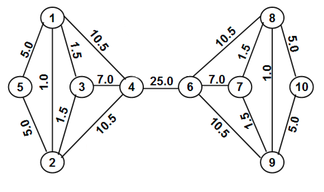
\includegraphics[scale=0.6]{pics/edge_betweenness_1}
	\end{center}
	\caption{Граф, для ребёр которого посчитаны значения Edge betweenness}
\end{figure}


В данном графе хочется выделить два сообщества: с вершинами 1-5 и 6-10. Граница же будет проходить через ребро, имеющее максимальный вес, 25. На этой идее и основывается алгоритм: поэтапно удаляем ребра с наибольшим весом, а оставшиеся компоненты связности объявляем сообществами.

Собственно, сам алгоритм \cite{edge_betweenness}:
\begin{enumerate}
\item Инициализировать веса
\item Удалить ребро с наибольшим весом
\item Пересчитать веса для ребёр
\item Сообществами считаются все компоненты связности
\item Посчитать функционал модулярности
\item Повторять с шаги 2-6, пока есть рёбра
\end{enumerate}

На каждой итерации процесса получается некое разбиение вершин. Последовательность таких разбиений, имеющая вид дерева, в листьях которого находятся сообщества с одной вершиной, а в корне --- большое сообщество, содержащее все вершины, называется дендрограммой. Результатом работы алгоритма является ярус дендрограммы (т.е. разбиение), имеющий максимальную модулярность. 

Из необходимости каждый раз пересчитывать веса следует главный минус: вычислительная сложность в худшем случае составляет $O(m^2n)$, где $m$ --- количество ребёр, $n$ --- количество вершин. Эксперименты показывают, что пересчитывать обычно приходится только веса для рёбер, которые были в одной компоненте связности, что несколько уменьшает сложность, однако зачастую этого оказывается недостаточно. 


\subsection{Label Propagation}
\label{sec:label_propagation}

Допустим, что большинство соседей какой-либо вершины принадлежат одному сообществу. Тогда, с высокой вероятностью, ему также будет принадлежать выбранная вершина. На этом предположении и строится алгоритм Label propagation: каждая вершина в графе определяется в то сообщество, которому принадлежит большинство его соседей. Если же таких сообществ несколько, то выбирается случайно одно из них. Пример:

\begin{figure}[h]
	\begin{center}
		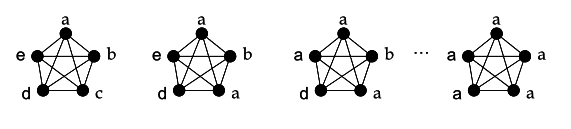
\includegraphics[scale=0.6]{pics/label_propagation}
	\end{center}
	\caption{Демонстрация работы алгоритма для полного графа}
\end{figure}

В начальный момент времени всем вершинам ставится в соответствие отдельное сообщество. Затем происходят перераспределения сообществ. Из-за случайности важно на каждой итерации изменять порядок обхода вершин. Алгоритм заканчивает работу, когда нечего изменять: все вершины относятся к тем сообществам, что и большинство их соседей. Авторы в \cite{label_propagation} также советуют запускать несколько раз алгоритм и выбирать наилучшее из результирующих разбиений, либо пересекать их. Главное достоинство данного алгоритма, в противовес предыдущему, --- почти линейная сложность. Однако на зашумленных графах зачастую происходит объединение всех вершин в одно сообщество. 


\subsection{FastGreedy}

Алгоритм \cite{fast_greedy} заключается в жадной оптимизации модулярности. Как и в прошлом методе, в каждой вершине графа инициализируется отдельное сообщество, а затем объединяются пары сообществ, приводящие к максимальному увеличению модулярности. При этом объединяются только инцидентные пары вершин, так как, в противном случае, модулярность не может увеличиться [во введении необходимо будет объяснить смысл модулярности, чтобы этот факт не вызывал вопросов]. 

Результатом работы алгоритма будет ярус дендрограммы, на котором модулярность максимальна.

Метод является вычислительно нетрудоёмким ($O(m\log n)$), легко применим к большим графам и, несмотря на жадность, зачастую неплохо справляется с задачей.

\subsection{WalkTrap}

Допустим, на вершинах графа задана такая метрика, что между двумя вершинами из разных сообществ расстояние велико, а из одного --- мало. Тогда выделение сообществ можно рассматривать как задачу кластеризации вершин. Попытаемся ввести такую метрику, используя случайные блуждания. Объект может переместиться из вершины $i$ в вершину $j$ с вероятностью $P_{ij} = \frac{A_{ij}}{d_i}$, где $A$ --- матрица смежности, $d_i$ --- степень $i$. То есть на каждом шаге равновероятно выбирается "сосед"\ вершины $i$. Таким образом определяется матрица переходов $P$ случайного блуждания. Она примечательна тем, что её степени являются вероятностями перехода из одной вершины в другую за соответствующее число шагов: вероятность перехода из $i$ в $j$ за $t$ шагов равна $(P^t)_{ij}$. Также следует отметить, что $P = D^{-1}A$, где $D$ --- матрица со степенями вершин на диагонали. Используя этот аппарат можно ввести желаемую метрику на вершинах: 
\[
r_{ij} = \sqrt{\sum\limits_{k=1}^{n}\frac{(P_{ik}^t - P_{jk}^t)^2}{d(k)}} = \bigl\|D^{-\frac{1}{2}}P^t_{i\bullet} - D^{-\frac{1}{2}}P^t_{j\bullet}\bigr\|,
\]
где $P^t_{i\bullet}$ --- вектор из вероятностей перехода за $t$ шагов из вершины $i$ во все другие. Вообще говоря, метрика зависит от $t$, авторы в \cite{walktrap} советуют брать $3 \leq t \leq 8$.

Естественным образом расстояние между вершинами обобщается на расстояние между сообществами:
\[
r_{C_1 C_2} = \bigl\|D^{-\frac{1}{2}}P^t_{C_1\bullet} - D^{-\frac{1}{2}}P^t_{C_2\bullet}\bigr\| = \sqrt{\sum\limits_{k=1}^{n}\frac{(P_{C_1k}^t - P_{C_2k}^t)^2}{d(k)}},
\]

где 
\[
P_{Cj}^t = \frac{1}{|C|}\sum\limits_{i\in C}P_{ij}^t
\]

Теперь, когда задана метрика, можно попытаться выделить кластеры в графе.
Начальное разбиение --- по одной вершине в каждом кластере $\mathcal{P}_1 = \{\{v\}, v\in V\}$. Также для всех пар инцидентных вершин считается расстояние. Далее для каждого k:
\begin{enumerate}
\item Выбрать $C_1$ и $C_2$ из $\mathcal{P}_k$ согласно некоторому метрическому критерию. 
\item Объединить два сообщества в новое $C_3 = C_1 \cup C_2$ и обновить разбиение $\mathcal{P}_{k+1} = (\mathcal{P}_k \setminus \{C_1, C_2\}) \cup C_3$.
\item Обновить расстояния между инцидентными сообществами.
\end{enumerate}

После $n-1$ шага получается дендрограмма разбиений, а $\mathcal{P}_n = \{V\}$. Таким образом, остался неясным только критерий выбора пар сообществ на шаге 1.
Будем выбирать пару сообществ, минимизирующих приращение среднего квадратов расстояний между каждой вершиной и их сообществом при объединении этих сообществ. Т.е.
\[
\Delta\sigma(C_1, C_2) = \frac{1}{n}\left(\sum\limits_{i\in C_3}r_{iC_3}^2 - \sum\limits_{i\in C_1}r_{iC_1}^2 - \sum\limits_{i\in C_2}r_{iC_2}^2 \right) \to \min\limits_{C_1, C_2}
\]
Теперь осталось только получить результат, выбрав разбиение, на котором достигает максимума модулярность.


\subsection{Infomap}

В данном методе применяется подход, основанный на случайных блужданиях и кодах Хаффмана. Напомним, что последние представляют из себя: если буквы в алфавите встречаются одинаково часто, то можно зафиксировать некоторую достаточную длину двоичного кода и кодировать сообщение последовательностью соответствующих двоичных блоков заданной длины. Однако, если, к примеру, одна буква встречается в три раза чаще другой, то использовать равномерный код нерационально с точки зрения итоговой длины сообщения. Эту проблему и решают коды Хаффмана: длина кода буквы в них обратно пропорциональна её частоте.

Вернёмся к сообществам. У каждой вершины есть некоторая вероятность её посещения. С помощью кодов Хаффмана, в соответствии с этими вероятностями, можно закодировать путь блуждателя. Эта последовательность будет иметь некоторую длину. Однако, если использовать иерархическое кодирование (т.е. кодируем сообщество, затем кодируем вершины, попавшие в это сообщество; коды вершин в разных группах могут совпадать), то можно сократить длину получившейся последовательности.

Как происходит иерархическое кодирование: при входе в сообщество записывается его уникальный код, затем записывается код вершины, в которую попали. Далее при переходах внутри сообщетсва пишутся только коды вершин. При выходе из сообщества пишется уникальный для него код выхода.

На этом и основывается метод Infomap \cite{infomap}: жадным способом минимизируется длина кода прогулки блуждателя.

Иллюстрация работы алгоритма:

\begin{figure}[h]
	\begin{center}
		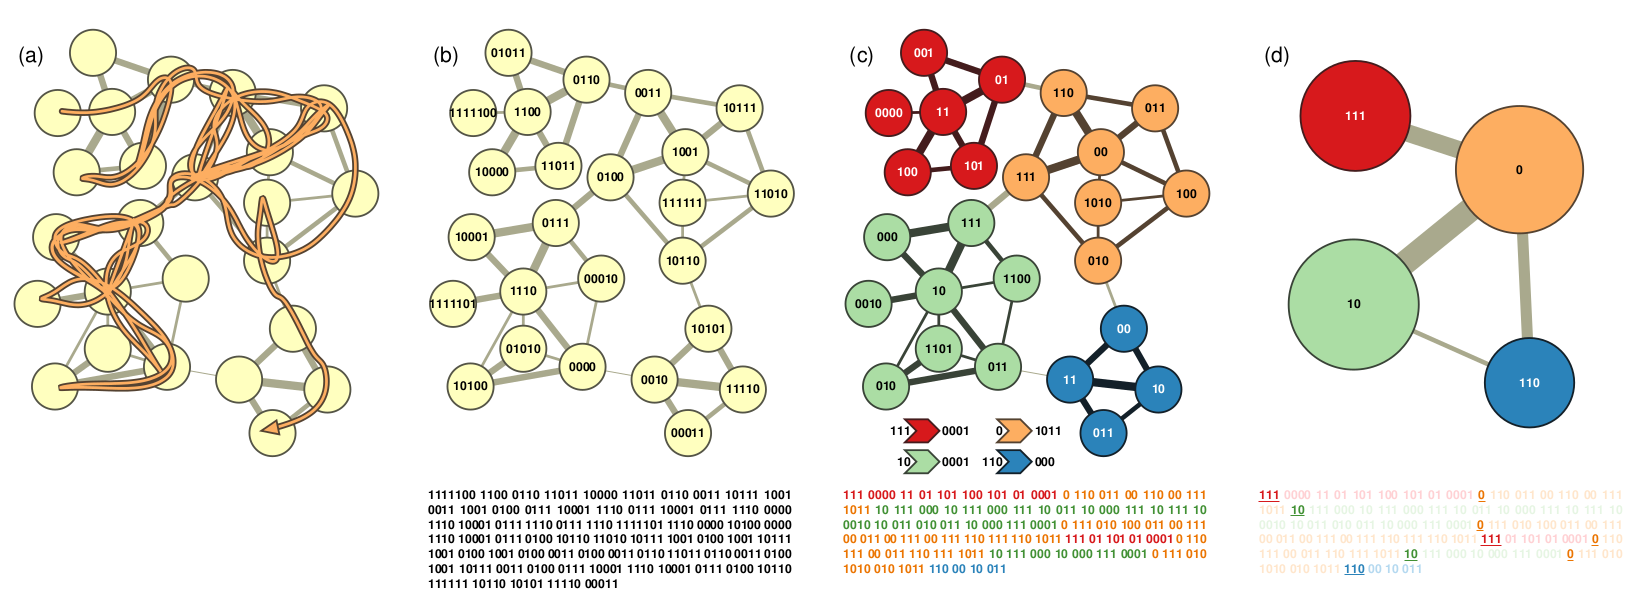
\includegraphics[scale=0.28]{pics/infomap}
	\end{center}
	\caption{На левом рисунке показан путь случайного блуждателя. На второй части изображены вершины с кодами Хаффмана, а ниже закодирован путь, изображенный на левом изображении. Далее показано кодирование с помощью иерархического метода. Ниже записаны коды сообществ и коды выхода из них. В самом низу закодирован путь. Длина кода уменьшилась. На последнем рисунке показаны сообщества и их коды}
\end{figure}

%Запишем формально среднюю длину одного перехода
%\[
%L(\mathcal{P}) = q_{\curvearrowright}H(\mathcal{P}) + \sum\limits_{i=1}%^mp_{\circlearrowright}^iH(C_i),
%\]
%где $q_{\curvearrowright}$ — вероятность покинуть какое-либо сообщество на любом шаге, $H(\mathcal{P})$ — энтропия кодов сообществ, $H(C_i)$ — энтропия кодов внутри сообщества $C_i$, вес $p_{\circlearrowright}^i$ это доля перемещений внутри сообщества $C_i$ плюс вероятность покинуть сообщество.

%Именно этот функционал и минимизируется.


\subsection{Leading Eigenvector}

Для начала небольшой экскурс по спектральным методам выделения сообществ. Допустим, для простоты, что всего в графе 2 группы. Тогда предлагается, согласно неформальному определению сообществ, что количество ребёр между этими группами, также называемое \textit{cut size},
\[
R = \frac{1}{2}\sum\limits_{\substack{i, j\ \text{в} \\ \text{разных} \\ \text{группах}}} A_{ij},
\]
должно быть мало.

Чтобы получить более удобное представление вводится вектор индексов $\bold s$ 
\[
s_i = 
\begin{cases}
+1, & \text{если вершина } i \text{ принадлежит сообществу 1} \\
-1, & \text{если вершина } i \text{ принадлежит сообществу 2}
\end{cases}
\]
с $n$ элементами.
Тогда
\[
\tfrac{1}{2}(1 - s_is_j) = 
\begin{cases}
1, & \text{если вершины } i \text{ и } j \text{ принадлежат разным группам} \\
0, & \text{если вершины } i \text{ и } j \text{ принадлежат одинаковым группам}
\end{cases}
\]
и величину \textit{cut size} можно переписать в виде
\[
R = \tfrac{1}{4}\sum\limits_{\substack{1 \leq i \leq n \\ 1 \leq j \leq n}}(1 - s_is_j)A_{ij}
\]
Используем следующую цепочку преобразований
\[
\sum\limits_{ij}A_{ij} = \sum\limits_{i}d_i = \sum\limits_{i}s_i^2d_i = \sum\limits_{ij}s_is_jd_i\delta_{ij}
\]
и перепишем \textit{cut size} следующим образом:
\[
R = \tfrac{1}{4}\sum\limits_{ij}s_is_j(d_i\delta_{ij} - A_{ij}) = \tfrac{1}{4}{\bold s}^T\textbf{Ls}
\]
где \textbf{L} --- матрица Лапласа с элементами
\[
L_{ij} = 
\begin{cases}
d_i, & \text{если } i = j \\
-1, & \text{если } i \neq j \text{ и между } i \text{ и } j \text{ есть ребро} \\
0, & \text{иначе}
\end{cases}
\]

Далее надо отметить несколько интересных нам свойств матрицы Лапласа:
\begin{enumerate}
\item Матрица симметричная, а, значит, из собственных векторов можно составить ортонормированный базис
\item Все собственные значения матрицы неотрицательны
\item Сумма по любой строке или по любому столбцу равна 0
\item Из свойств 2 и 3 следует, что всегда будет нулевое собственное значение и соответствующий ему собственный вектор $(1, 1, 1, \dots) / \sqrt{n}$
\end{enumerate}

Можно пойти дальше и ещё упростить запись \textit{cut size}: если разложить $\textbf{s} = \sum_{i=1}^na_i\textbf{v}_i$, где $\textbf{v}_i$ --- собственный вектор $\textbf{L}$, $a_i = \langle\textbf{v}_i, \textbf{s}\rangle$, то 
\[
R = \sum\limits_ia_i\textbf{v}^T_i\textbf{L}\sum\limits_ja_j\textbf{v}_j = \sum\limits_{ij}a_ia_j\lambda_j\delta_{ij} = \sum\limits_ia_i^2\lambda_i
\]

Таким образом, минимизацию $R$ можно рассматривать как выбор $a_i^2$, минимизирующих сумму. Как было отмечено, всегда существует собственный вектор из единиц. Если положить $\textbf{s} = (1, 1, 1, \dots)$, то $R$ становится равным нулю, что соответствует объединению всех вершин в одно сообщество. Такой тривиальный случай нас не интересует, поэтому рассматривается собственный вектор, соответствующий второму минимальному собственному значению. То есть мы будем подбирать вектор $\textbf{s}$ наиболее близким к $\textbf{v}^{(2)}$. Учитывая ограничение, что значения $\textbf{s}$ могут быть только $\pm1$, искомое $\textbf{s}$ принимает вид
\[
s_i = 
\begin{cases}
+1, & v^{(2)}_i \geq 0 \\
-1, & v^{(2)}_i < 0
\end{cases}
\]

Это и есть спектральный метод в простейшем виде.

Однако автор в \cite{leading_eigenvector} отмечает, что хорошее разделение --- не совсем то, через которое проходит наименьшее число вершин. Он предлагает разделять те места, где количество рёбер меньше, чем ожидалось, или, наоборот, объединять те вершины, у которых количество рёбер больше, чем ожидалось:
\[
Q = (\text{количество вершин внутри сообщества}) - (\text{ожидаемое количество вершин})
\]
\[ = \frac{1}{2m}\sum_{i,j}\left(A_{ij}-\frac{d_i d_j}{2m}\right)\delta(C_i, C_j) \to \max,
\]
что в точности является функционалом модулярности. Именно Ньюманом и Гирваном ранее в их работах она впервые была предложена.

Используя $\delta(C_i, C_j) = \tfrac{1}{2}(s_is_j+1)$ перепишем
\[
Q = \frac{1}{4m}\sum_{i,j}\left(A_{ij}-\frac{d_i d_j}{2m}\right)(s_is_j+1) = \frac{1}{4m}\textbf{s}^T\textbf{Bs},
\]
где \textbf{B}, называемая матрицей модулярности, во многих смыслах похожа на матрицу Лапласа
\[
B_{ij} = A_{ij} - \frac{d_i d_j}{2m}
\]

И именно настраивая вектор \textbf{s} на собственный вектор, соответствующий максимальному собственному значению, получается метод Leading Eigenvector.
\[
s_i = 
\begin{cases}
+1, & u^{(1)}_i \geq 0 \\
-1, & u^{(1)}_i < 0
\end{cases}
\]

Напомним, что будет относить к сообществу 1 те вершины, у которых соответствующее значение вектора \textbf{s} равно плюс единице, и к сообществу 2 иначе. Подобным образом граф разбивается на сообщества, пока увеличивается значение модулярности.


\subsection{MultiLevel}

\begin{figure}[h]
	\begin{center}
		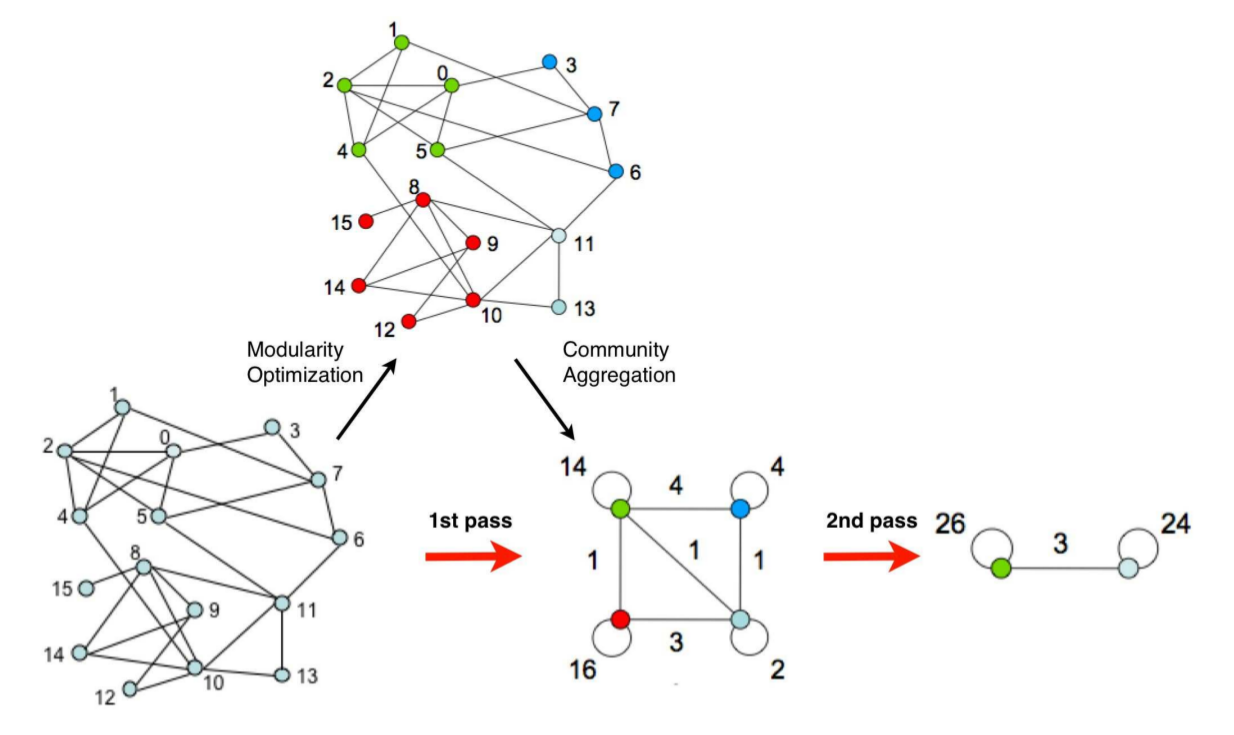
\includegraphics[scale=0.3]{pics/multilevel}
	\end{center}
	\caption{Илюстрация работы алгоритма Multilevel: два прохода, для первого показаны оба этапа}
\end{figure}

Алгоритм \cite{multilevel} основан на оптимизации модулярности. Как и в многих предыдущих методах, каждой вершине сначала ставится в соответствие по сообществу. Далее чередуются следующие этапы:
\begin{enumerate}
\item Первый этап
\begin{itemize}
\item Для каждой вершины перебираем её соседей
\item Перемещаем в сообщество соседа, при котором модулярность увеличивается максимально 
\item Если перемещение в любое другое сообщество может только уменьшить модулярность, то вершина остаётся в своём сообществе
\item Последовательно повторяем, пока какое-либо улучшение возможно
\end{itemize}
\item Второй этап
\begin{itemize}
\item Создать метаграф из сообществ-вершин. При этом рёбра будут иметь веса, равные сумме весов всех рёбер из одного сообщества в другое или внутри сообщества (т.е. будет взвешенная петля)
\item Перейти на первый этап для нового графа
\end{itemize}
\end{enumerate}

Алгоритм прекращает работу, когда на обоих этапах модулярность не поддаётся улучшению. Все исходные вершины, которые входят в финальную метавершину, принадлежат одному сообществу.

Несколько замечаний: 
\begin{itemize}
\item На первом этапе вершина может рассматриваться несколько раз
\item Порядок перебора не сильно влияет на точность, однако может существенно влиять на время работы алгоритма
\item На практике оказывается достаточно 3-4 итераций
\end{itemize}

\newpage


\section{Разбиение на пересекающиеся сообщества}

\subsection{k-Clique Perlocation}

Clique perlocation method (CPM) основан на предположении, что сообщества состоят из пересекающихся полных подграфов. Алгоритм начинает работу с поиска всех клик размера $k$, после чего строится новый граф, вершинами которого являются найденные клики. Ребро образуется в случае, если пересечение вершин-клик состоит из  $k-1$ вершины исходного графа. Компоненты связности нового графа и будут определять найденные сообщества. Эксперименты в \cite{cpm} показывают, что k хорошо брать в пределах от 3 до 6. Метод хорош своей интуитивностью, однако неприменим на графах с очень большим количеством вершин.

\subsection{BigCLAM}

Cluster Affiliation Model for Big Networks --- вероятностная генеративная модель, сводящая задачу выделения сообществ к задаче неотрицательной матричной факторизации \cite{bigclam}. Для начала немного изменим исходную постановку: теперь у нас будет двудольный граф, в одной доле которого находятся сообщества, а в другой --- вершины, причём каждая вершина $u \in V$ не просто принадлежит сообществу $c \in C$, а принадлежит ему с каким-то неотрицательным весом $F_{uc}$ (если не принадлежит, то вес равен нулю):

\begin{figure}[h]
	\begin{center}
		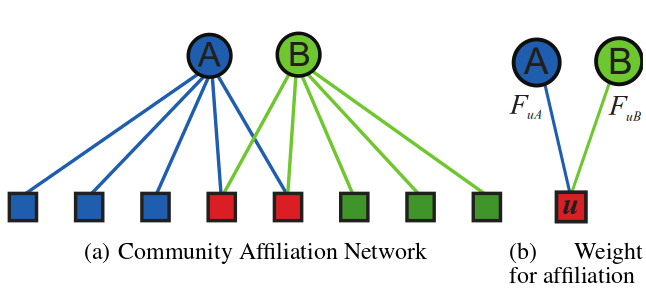
\includegraphics[scale=0.33]{pics/cluster_affiliation}
	\end{center}
	\caption{Двудольный граф принадлежностей. Рёбра с нулевыми весами не отображаются}
\end{figure}

Тогда, для заданной матрицы весов $F$ предполагается, что каждое сообщество соединяет вершины $u$ и $v$ с вероятностью $1 - \exp(-F_{uc}\cdot F_{vc})$. Для всех сообществ вероятность ребра между $u$ и $v$ равна $1 - \exp(-\sum_c F_{uc} \cdot F_{vc})$ или, в краткой форме,
\[
p(u, v) = 1 - \exp(-F_{u} \cdot F_{v}^T). 
\]

Теперь можно воспользоваться методом максимизации правдоподобия: для заданного графа $G(V, E)$ будем стараться найти $K$ сообществ, при которых $\hat F \in \mathbb{R}^{N \times K}$ доставляет максимум правдоподобия:
\[
\hat F = \arg\max_{F: F_{uc} \geq 0} l(F)
\]
\[
l(F) = \log P(G|F) = \sum\limits_{(u, v) \in E} \log (1 - \exp(-F_u \cdot F_v^T)) - \sum\limits_{(u, v) \notin E} F_u \cdot F_v^T
\]

Эта задача оптимизации и сводится к неотрицательной факторизации матрицы смежности $A$ графа $G$. Определять $K$ предлагается по значению правдоподобия на отложенной выборке (на 20\% выбранных вершин исходного графа). 

В итоге получается матрица $F$ степеней принадлежностей вершин сообществам. Результирующая принадлежность (принадлежит/не принадлежит) определяется отсечением по порогу.

Осталось лишь описать поиск $F$. Будем использовать блочно-координатный градиентный метод. Предлагается обновлять каждое $F_u$ при фиксированных остальных $F_v$, то есть обновлять принадлежности конкретной вершины при фиксированных принадлежностях других. Главная причина фиксации: задача становится выпуклой. То есть, для каждой вершины $u$ решается вспомогательная задача: 
\[
\hat F_u = \arg\max_{F_{uc} \geq 0} l(F_u),
\]
где
\[
l(F_u) = \sum\limits_{v \in \mathcal{N}(u)} \log (1 - \exp(-F_u \cdot F_v^T)) - \sum\limits_{v \notin \mathcal{N}(u)} F_u \cdot F_v^T,
\]
где $\mathcal{N}(u)$ --- множество соседей вершины $u$. Именно благодаря суммированию только по соседям метод получается очень масштабируемым: реальный социальные графы больших размеров очень разреженные, то есть вершины имеют малое по сравнению с количеством вершин в графе количество соседей, вследствие чего каждое обновление имеет близкую к константе вычислительную сложность.

\subsection{DEMON}

Алгоритм Democratic Estimate of the Modular Organization of a Network \cite{demon} является обобщением метода Label Propagation, описанного \hyperref[sec:label_propagation]{ранее}. Сначала для каждой вершины $v$ стоится эго-сеть: выбирается подграф, вершинами которого являются соседи $v$, а рёбрами --- все рёбра между всеми соседями $v$. Далее, для данной эго-сети запускается Label Propagation, в результате работы которого получается некоторое разбиение $\mathcal{C}(v)$ на сообщества соседей $v$. После этого его необходимо объединить с итоговым покрытием $\mathcal{C}$, которое инициализируется пустым. Опишем, как происходит объединение. Два сообщества $I$ и $J$ объединяются в том и только в том случае, если не более $\varepsilon$ процентов меньшего из них не содержится в большем из них. Например, для $\varepsilon = 0$ объединение будет происходить только, когда одно из сообщетсв полностью содержится в другом, а для $\varepsilon = 1$ объединение будет происходить всегда. Теперь можем описать сам алгоритм:
\begin{enumerate}
\item Инициализировать $\mathcal{C} = \emptyset$
\item Для вершины $v \in V$ построить эго-сеть и получить её разбиение $\mathcal{C}(v)$ с помощью Label Propagation
\item Для каждого из сообществ в $\mathcal{C}(v)$ и для каждого из сообществ в $\mathcal{C}$ произвести объединение с заданным порогом.
\item Повторять шаги 2-4, пока есть нерассмотренные вершины.
\end{enumerate}

\subsection{CONGO}

Сluster-Overlap Newman Girvan Optimized аlgorithm также является обобщением ранее описанного метода, а именно \hyperref[sec:edge_betweenness]{Edge Betweenness}. Автор вводит дополнительную операцию разбиения вершины для того, чтобы результатом было разбиение на пересекающиеся сообщества. Раньше каждому ребру ставилось в соответствие значение edge betweenness, с помощью которого происходило последовательное удаление рёбер (удалялось ребро с максимальным edge betweenness, после чего значения пересчитывались). Теперь дополнительно каждой вершине будем ставить в соответствие величину split betweenness. Представим, что вершину $v$ заменили на $v1$ и $v2$. Тогда split betweenness вершины $v$ будет равен количеству кратчайших путей, проходящих через виртуальное ребро между $v1$ и $v2$. При этом смежные с $v$ рёбра делятся между $v1$ и $v2$ таким образом, чтобы величина split betweenness была максимальной для $v$. Пример:
\begin{figure}[h]
	\begin{center}
		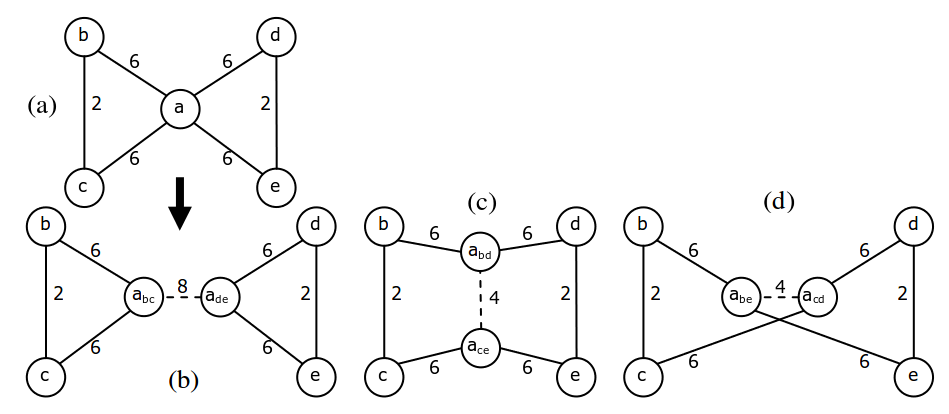
\includegraphics[scale=0.4]{pics/split_betweenness}
	\end{center}
	\caption{(a) Граф. (b) Лучшее разбиение вершины a. (c), (d) Другие разбиения.}
\end{figure}

Далее последовательно повторяются удаления рёбер и разбиения вершин. Однако автор в \cite{congo} отмечает, что после каждой такой операции пересчитывать значения split и edge betweenness очень дорого, так как приходится "проходиться"\ по всему графу. Поэтому предлагается пересчитывать значения betweenness только для путей, длина которых не превосходит некоторого h, являющегося параметром алгоритма.
Итоговый алгоритм:
\begin{enumerate}
\item Посчитать все edge betweenness для рёбер и split betweenness для вершин
\item Найти ребро или вершину с максимальным значением betweenness
\item Удалить выбранное ребро или разбить выбранную вершину
\item Пересчитать величины betweenness в h-окрестности данного ребра или данной вершины
\item Повторять шаги 2-5, пока есть рёбра
\end{enumerate}

\section{Эксперименты}

\subsection{Данные}

Для начала будем пробовать методы на модельных данных. Создадим граф с $l$ сообществами, каждое из которых имеет по $g$ вершин. При этом рёбра будут генерироваться случайно: с вероятностью $p_{in}$ ребро появляется между вершинами из одного сообщества, с вероятностью $p_{out}$ --- между вершинами из разных. В наших экспериментах возьмём $l = 4, g = 64, p_{in} = 0.5$, а величину $p_{out}$ будем варьировать, постепенно зашумляя граф и смотря на зависимость качества методов от зашумлённости графа. На этих данных будем тестировать методы для обнаружения непересекающихся сообщетсв. Стоит отметить, что в данном случае мы знаем истинное разбиение на сообщества (ground truth), поэтому будут использоваться метрики при известных ответах, которые будут описаны ниже.

Реальные данные возьмём из соревнования Learning Social Circles in Networks \cite{kaggle} с платформы kaggle, представляющие из себя 110 эго-сетей (граф, вершинами которого являются друзья пользователя, а рёбрами --- связи между ними, в случае из начилия). На этих сетях также будем тестировать методы для обнаружения пересекающихся сообществ, однако истинные разбиения неизвестны, поэтому будут использоваться соответствующие метрики. 

Наконец, данными для пересекающихся сообществ будут также эго-сети пользователей Facebook, для всех вершин каждой из которых известны принадлежности сообществам.

\subsection{Метрики качества}

\subsubsection*{Normalized Mutual Information}

Если два разбиения похожи, то требуется небольшое количество информации, чтобы восстановить одно из разбиений по другому. Эта идея и лежит в основе метрики NMI, которая является мерой непохожести разбиений (мерой похожести тогда будет являться $1 -$NMI).

Представим себе два разбиения $\{x_i\}$ и $\{y_i\}$, где i --- номер вершины, а $x_i$ и $y_i$ --- соответствующие им номера сообществ. Также представим, что метки $x$ и $y$ --- значения случайных величин $X$ и $Y$, имеющих совместное распределение $P(X = x, Y = y) = \frac{n_{xy}}{n}$, где $n$ --- общее количество вершин, а $n_{xy}$ --- количество вершин, которые в разбиениях $\{x_i\}$ и $\{y_i\}$ имеют метки $x$ и $y$. Аналогично $P(X = x) = \frac{n_{x}}{n}$, $P(Y = y) = \frac{n_{y}}{n}$. 

Напомним определение энтропии и условной энтропии распределения:
\[
H(X) = -\sum\limits_x P(x)\log P(x),\qquad H(X|Y) = -\sum\limits_{x, y} = P(x, y)\log P(x|y)
\]

Тогда взаимная информация будет определяться как их разность:
\[
I(X, Y) = H(X) - H(X|Y), 
\]
а нормировка производится на сумму отдельных энтропий:
\[
I_{norm}(X, Y) = \frac{I(X, Y)}{H(X) + H(Y)}
\]

Эта метрика будет использоваться как для непересекающихся, так и для пересекающихся сообществ с ground truth.

\subsubsection*{Split-Join Distance}

Эта метрика является аналогом редакторского расстояния для разбиений: она измеряет минимальное количество операций, необходимых для перехода от одного разбиения к другому. Операциями могут быть:
\begin{itemize}
\item Добавить вершину к сообществу
\item Удалить вершину из сообщества
\item Создать сообщество с одной вершиной
\item Удалить сообщество с одной вершиной
\end{itemize}

Эта метрика будет использоваться для непересекающихся сообществ с ground truth.

\subsubsection*{Modularity}

Значения функционала модулярности, который многократно упоминался ранее, будем смотреть для эго-сетей с kaggle как меру правильности работы алгоритмов обнаружения непересекающихся сообществ для неразмеченных данных.

\subsubsection*{Omega Index}

Omega Index измеряет количество согласованных пар вершин в двух покрытиях графов. Две вершины назовём соглаванными, если они лежат в одинаковом количестве сообществ. То есть, Omega Index считает, сколько пар вершин принадлежат одновременно одному сообществу, двум сообществам и так далее.

Пусть $K_1$ и $K_2$ --- количество сообществ в покрытиях $C_1$ и $C_2$ соответственно. Тогда 
\[
\omega(C_1, C_2) = \frac{\omega_u(C_1, C_2) - \omega_e(C_1, C_2)}{1 - \omega_e(C_1, C_2)},
\]
где 
\[
\omega_u(C_1, C_2) = \frac{1}{M}\sum\limits_{j=0}^{max(K_1, K_2)}|t_j(C_1)\cap t_j(C_2)|,
\]
\[
\omega_e(C_1, C_2) = \frac{1}{M^2}\sum\limits_{j=0}^{max(K_1, K_2)}|t_j(C_1)|\cdot |t_j(C_2)|.
\]
Здесь $M$ равно $n(n-1)/2$ --- количество пар вершин, а $t_j(C)$ --- множество пар вершин, которые встречаются в покрытии $C$ ровно $j$ раз.

Omega Index равен единице, только в случае, если $\omega_u(C_1, C_2)$ равен единице, что означает точное совпадение $C_1$ и $C_2$.

Эта метрика будет использоваться для пересекающихся сообществ с ground truth.

\subsection{Результаты}

\begin{figure}[h]
	\begin{minipage}{0.5\textwidth}
		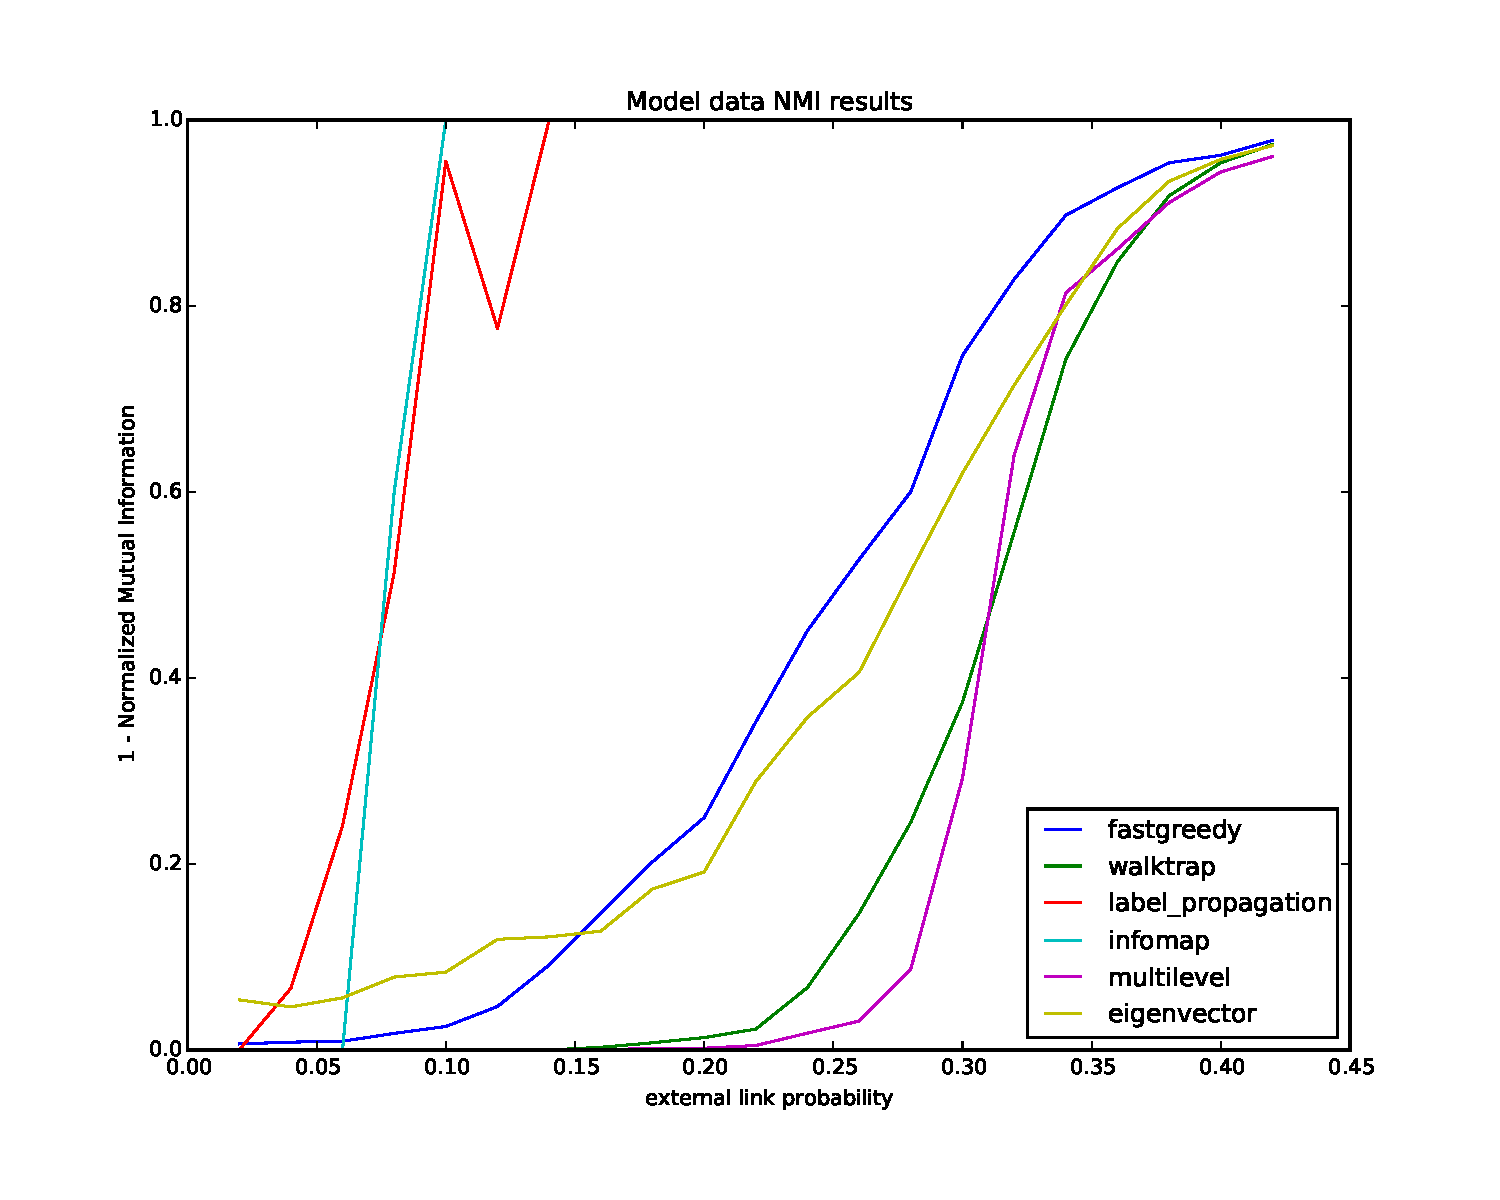
\includegraphics[scale=0.345]{pics/model_data_nmi}
	\end{minipage}
	\begin{minipage}{0.5\textwidth}
		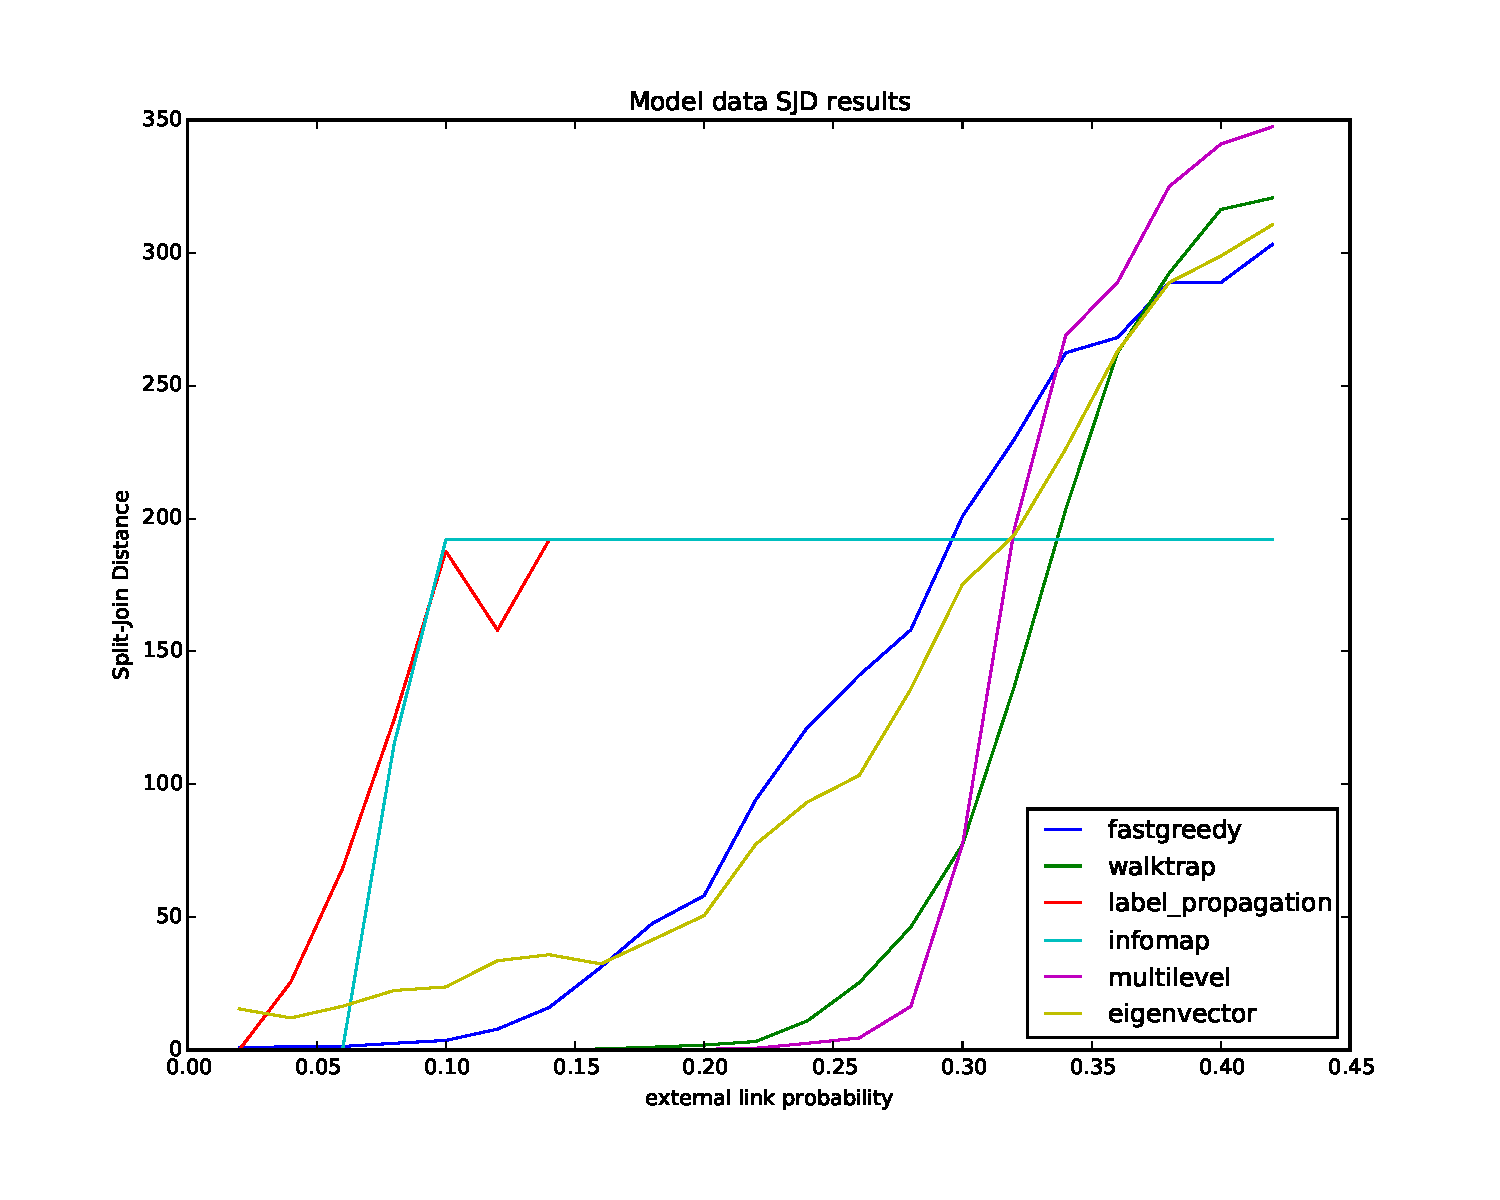
\includegraphics[scale=0.345]{pics/model_data_sjd}
	\end{minipage}
	\caption{Результаты работы методов обнаружения непересекающихся сообществ на модельных данных \label{fig::model_data_results}}
\end{figure}

Метод Edge Betweenness показал непозволительно высокую вычислительную сложность (более, чем в 10 раз дольше любого другого алгоритма) даже на простых модельных данных, поэтому из испытаний был исключён. Алгоритмы Label Propagation и Infomap таким недостатком не обладали, однако оказались крайне чувствительны даже к небольшому шуму. Лучше всего с задачей справились методы MultiLevel и WalkTrap: рис. \ref{fig::model_data_results}.

\begin{figure}[h]
	\begin{center}
		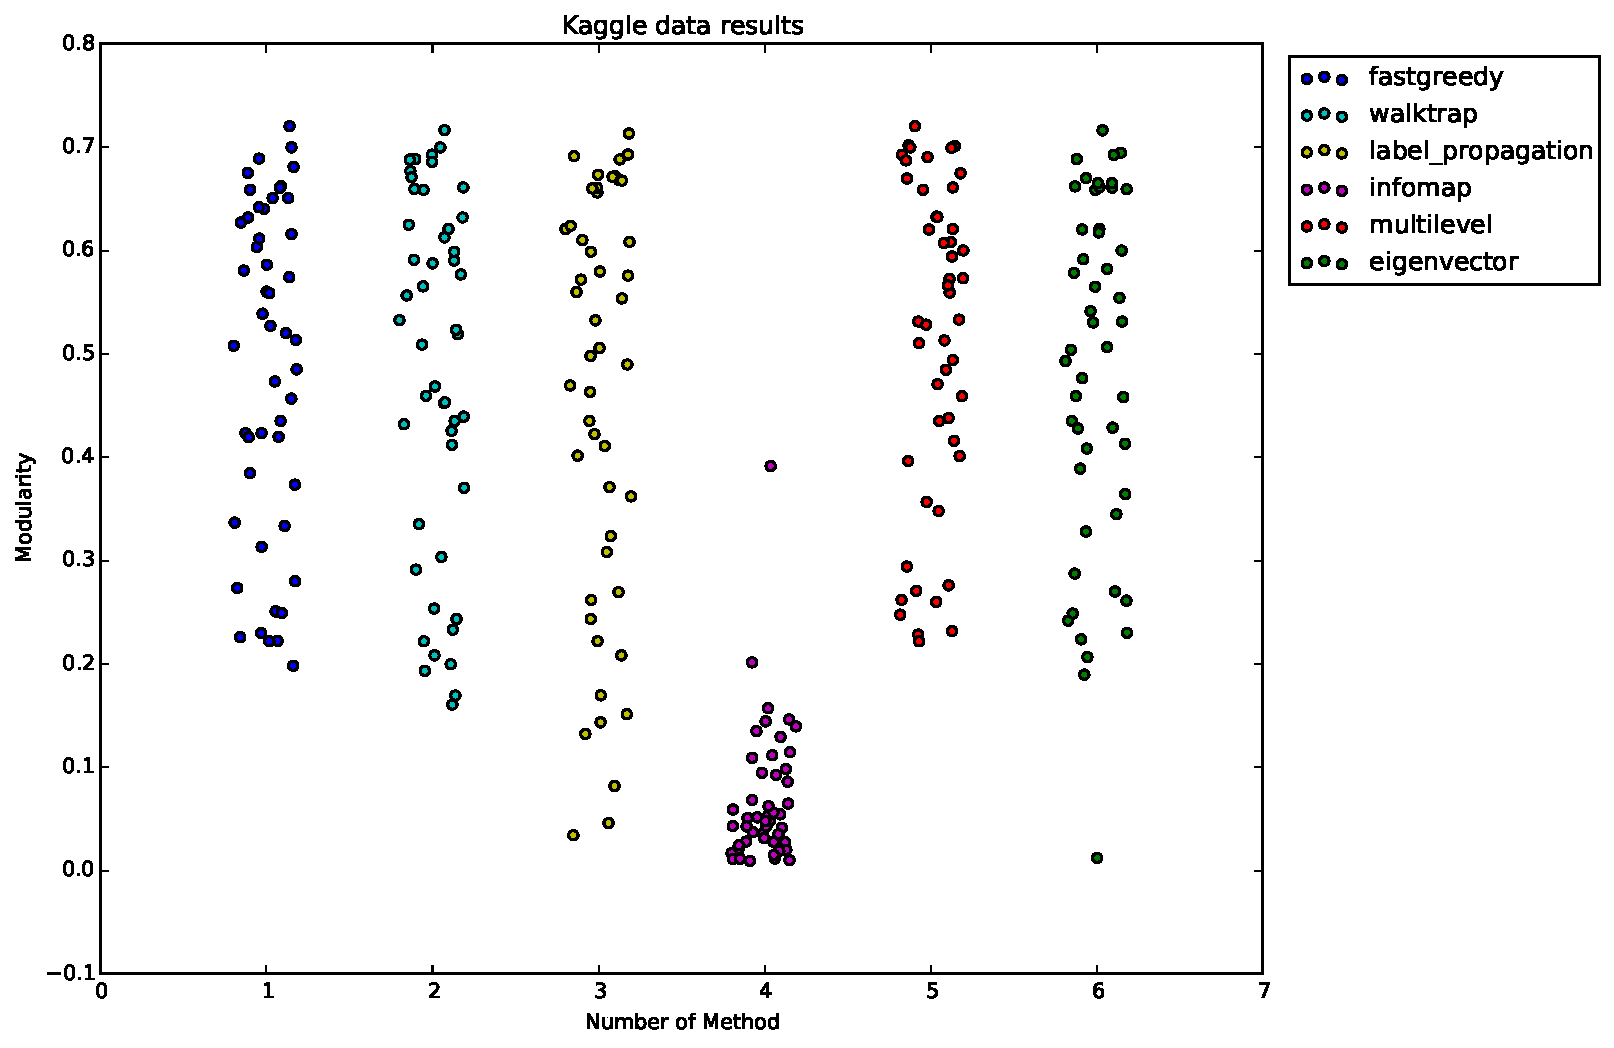
\includegraphics[scale=0.35]{pics/kaggle_modularity}
	\end{center}
	\caption{Результаты работы методов обнаружения непересекающихся сообществ на реальных эго-сетях. Точкой обозначается результат на отдельной эго-сети. Ось абсцисс введена искусственно для удобства читателя \label{fig::modularity_kaggle}}
\end{figure}

На реальных данных метод Label Propagation оказался не так плох, как на модельных, в отличие от Infomap, который снова не справился с задачей. В среднем, MultiLevel справился лучше других методов: рис. \ref{fig::modularity_kaggle}. Все методы, за исключением Edge Betweenness, отработали и на синтетических, и на реальных данных очень быстро.

\begin{figure}[h]
\begin{center}
\begin{tabular}{rr|rrrr}
\hline
\multicolumn{2}{c|}{Различные эго-сети} & \multicolumn{4}{c}{$1 -$NMI}\\
\hline
 \# вершин &  \# рёбер &  BigCLAM &     CPM &   CONGO &   DEMON \\
\hline
       59 &    146 &   0.2497 &  \bf{0.2975} &  0.1703 &  0.2315 \\
       66 &    270 &   0.3580 &  \bf{0.4305} &  0.3513 &  \bf{0.4305} \\
      159 &   1693 &   0.2898 &  0.3454 &  0.3278 &  \bf{0.4057} \\
      170 &   1656 &   0.1460 &  \bf{0.2730} &  0.1381 &  0.1585 \\
      227 &   3192 &   0.2342 &  \bf{0.2700} &  0.2366 &  0.2408 \\
      347 &   2519 &   \bf{0.0501} &  0.0476 &  0.0477 &  0.0489 \\
      547 &   4813 &   0.0120 &  0.0157 &  0.0241 &  \bf{0.0400} \\
      755 &  30025 &   0.1207 &  Memory &  Time &  \bf{0.1821} \\
      792 &  14024 &   0.2401 &  Memory &  Time &  \bf{0.3620} \\
     1045 &  26749 &   \bf{0.1382} &  Memory &  Time &  0.1245 \\
\hline
\end{tabular}
\caption{$1 -$Normalized Mutual Information для методов обнаружения пересекающихся сообществ. Memory --- метод оказался слишком сложным по памяти. Time --- метод не сошелся за приемлемое время \label{fig::nmi_overlap}}
\end{center}
\end{figure}

\begin{figure}[h]
\begin{center}
\begin{tabular}{rr|rrrr}
\hline
\multicolumn{2}{c|}{Различные эго-сети} & \multicolumn{4}{c}{Omega Index}\\
\hline
 \# вершин &  \# рёбер &  BigCLAM &     CPM &   CONGO &   DEMON \\
\hline
        59 &         146 &   0.1058 &  \bf{0.1835} &  0.1299 &  0.0939 \\
        66 &         270 &   0.3307 &  0.3001 &  \bf{0.4413} &  0.3001 \\
       159 &        1693 &   0.3266 &  0.2622 &  \bf{0.3376} &  0.1521 \\
       170 &        1656 &   0.0521 &  \bf{0.0914} &  0.0749 &  0.0319 \\
       227 &        3192 &   0.0000 &  0.1793 &  0.0488 &  \bf{0.1817} \\
       347 &        2519 &   0.1257 &  \bf{0.2424} &  0.0619 &  0.1681 \\
       547 &        4813 &   \bf{0.0518} &  0.0080 &  0.0045 &  0.0043 \\
       755 &       30025 &   \bf{0.3917} &  Memory &  Time &  0.0000 \\
       792 &       14024 &   \bf{0.3378} &  Memory &  Time &  0.0181 \\
      1045 &       26749 &   \bf{0.1936} &  Memory &  Time &  0.0000 \\
\hline
\end{tabular}
\caption{Omega Index для методов обнаружения пересекающихся сообществ \label{fig::omega_overlap}}
\end{center}
\end{figure}

Как видно на рисунках \ref{fig::nmi_overlap}, \ref{fig::omega_overlap}, методы показали себя достаточно разнородно. Хочется отметить, что BigCLAM оказался действительно хорошо масштабируемым, практически не имел сложности по памяти и был очень быстр. Также неплох по всем этим параметрам оказался алгоритм DEMON. Весьма плохо и долго работал на всех данных CONGO, даже несмотря на название описывающей его статьи "A Fast Algorithm to Find Overlapping Communities in Networks". Clique Perlocation Method, в целом, показал себя неплохо на небольших сетях, однако при увеличении количества рёбер переставал справляться с задачей.

\subsection{Описание реализаций}

Использовался язык программирования Python 2. Для работы с графами, в основном, использовалась библиотека igraph \cite{igraph}. Изредка использовалась библиотека networkx \cite{networkx}.
Методы и метрики для выделения непересекающихся сообществ могут быть найдены в библитеке igraph. Для пересекающихся нет централизованной библиотеки, поэтому всё собиралось из различных источников, а именно:
\begin{itemize}
\item Библиотека Circulo \cite{circulo}, в которой могут быть найдены методы BigCLAM, Clique Perlocation и CONGO, приспособленные для библиотек igraph и networkx
\item Метрика NMI (для пересекающихся) бралась отсюда \cite{nmi}
\item Omega Index бралась отсюда \cite{omega}
\item Алгоритм DEMON \cite{demon_implementation}
\item Эго-сети Facebook брались из Stanford Network Analysis Platform (SNAP) \cite{snap}

Часть экспериментов может быть найдена на GitHub странице автора \cite{my_github}.
\end{itemize}

\section{Заключение}

В работе были рассмотрены методы выделения сообществ в социальных графах для непересекающихся и пересекающихся случаев. Стоит повторить, что выделение сообществ не является строгой задачей, хотя бы потому, что нет чёткой постановки задачи, вследствие чего нет идеального алгоритма. 

Описанные эксперименты позволяют выбрать алгоритм исходя из требований задачи: может быть необходима скорость работы, либо необходимо найти лучшее в некотором смысле разбиение, невзирая на вычислительные сложности, либо же граф может быть настолько большим, что большинство методов справиться с ним не может. 

%\vspace{2cm}
%2do: не забыть выровнять рисунки
%2do: разобраться с русской кодировкой и правильным оформлением списка литературы
%2do: замечания в блокноте

\bibliographystyle{gost780s}
\bibliography{references}

\end{document}
